\section{Methods}
\subsection{Metrics}
The metric chosen for the following experiments was accuracy, due to its comprehensible nature. Despite the fact that an unbalanced dataset presents one of the significant drawbacks of using accuracy, this concern is irrelevant in the case of MNIST since it is a balanced dataset. The accuracy of each node is computed after each training step using the test subset of MNIST, and none of the nodes are ever provided access to the test set for training.

\subsection{Data Collection}
The training process for each experiment was conducted five times, and the resulting accuracies of every node were recorded. To mitigate the impact of training noise on the performance graphs, the accuracy value for each time step was calculated as the median accuracy across all nodes and runs at that time step.

\subsection{Node Counts}
The experiments were conducted using 10 nodes, with the exception of the server in cases where FL was employed. The decision of how many nodes to simulate was based on the highest node count attainable without causing inconsistencies and crashes due to resource depletion of the training machine.

\subsection{Algorithm Configurations}
In each of the following experiments, the algorithm was configured using a specific set of parameters $\alpha \beta \gamma$. These parameters were obtained heuristically by making an initial guess, testing, and then fine-tuning them until a satisfactory outcome was reached. However, it is important to note that an exhaustive investigation into the optimal parameter configuration for a particular type of problem is not within this papers scope, meaning that it is plausible that swarm learning could yield better results with more precisely tuned parameters.

\subsection{Data Volume Per Node}
The experiments evaluate the algorithm's performance using three levels of data volume per node. These levels are considerably smaller than the full MNIST dataset not only to increase problem difficulty, but also as the algorithm is intended for scenarios where each nodes access to data is restricted. To create a subsection of data for each node, a random sampling with replacement method was used to select the desired number of datapoints. During the initial training phase, each node performs a single sampling of its dataset, after which that nodes data subset remains constant.

\subsection{Epochs}
Due to the limited size of the dataset, a single node executes more than one epoch of training in each training loop. The number of epochs carried out by a node per training step will be referred to as Epochs per Step (EPS). Empirical testing has indicated that both SL and FL exhibit improved performance with higher EPS, at times surpassing the gains from increasing the number of training steps. Moreover, the utilization of higher EPS was favoured due to its reduced training time, compared to increasing the number of training steps. The three levels of data volume with their respective EPS are shown in table \ref{epsparams}

\begin{table}[H]
	\begin{tabular}{p{1.5cm}|l|p{10cm}}
		Dataset Size & EPS & Reason \\ \hline \hline
		6000  & 2  & As there are 10 nodes, it was decided that each node should be tested with 1/10th of the dataset \\ \hline
		1000   & 5   & A much lower volume of data was tested to reflect the anticipated use case of SL - training models where each node has very small amounts of data \\ \hline
		100  & 15  & The extreme case was tested to see how well the algorithms perform in undesirable conditions	\end{tabular}
	\caption{The different levels of dataset size and EPS that were tested} \label{epsparams}
\end{table}

\section{Dense Network Performance}
A crucial experiment for evaluating the performance of the SL algorithm involves assessing its performance under optimal circumstances, specifically within a network of nodes wherein each node is directly connected to every other node. In FL, the analogous topology involves direct connections between each node and the server. This comparison is significant as it facilitates a direct evaluation of the SL and FL algorithms under their respective ideal conditions.

The selection of the parameters for the SL algorithm was based on the authors prior experience in testing the algorithm. These parameters are presented in Table \ref{slparamsDNP}.
\begin{table}[H]
	\begin{tabular}{p{0.5cm}|l|p{11cm}}
		P & Value & Reason \\ \hline \hline
		$\alpha$  & 0.75  & Low enough to allow nodes to maintain a small variation but not so low that the nodes diverge indefinitely                               \\ \hline
		$\beta$   & 0.5   & Allows a small amount of nodes looking back, but high value is not needed as every node will be running at approximately the same speed. \\ \hline
		$\gamma$  & 8     & All nodes will always be connected to 9 other nodes, so higher is better. There is room for 1 node to be skipped to prevent deadlock.   
	\end{tabular}
	\caption{The chosen parameters for the SL algorithm} \label{slparamsDNP}
\end{table}

\subsection{Results}
The following are the results obtained from the execution of the training script. Each graph displays the data for \SL in red, and FedAvg in black. The shaded region surrounding each line represents the upper and lower quartile.

\begin{figure}[H] 
	\center{\textbf{Accuracy by Training Step for 6000 Samples}} \\
	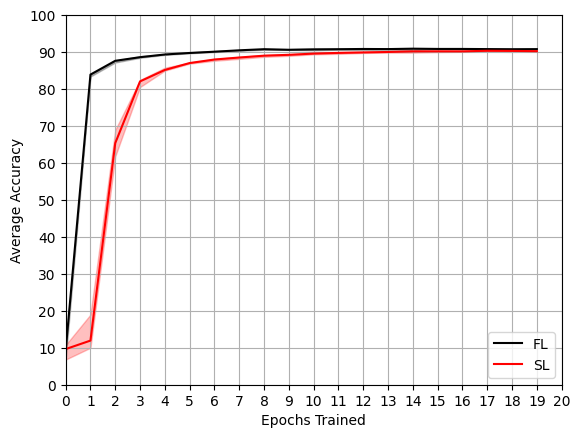
\includegraphics[width=300px]{aeg1}
	\caption{Comparing Accuracy of FL and SL with 6000 Data Samples per Node}
	\label{aeg1}
\end{figure}

The results depicted in Figure \ref{aeg2} demonstrate that the \SL algorithm exhibits a slower convergence rate compared to FedAvg. Despite this, both methods ultimately achieve a similar level of accuracy. Notably, the primary distinction between these two algorithms lies in the fact that \SL performs slightly worse than FedAvg, trailing by 1-2 epochs.

\begin{figure}[H]
	\center{\textbf{Accuracy by Training Step for 1000 Samples}} \\
	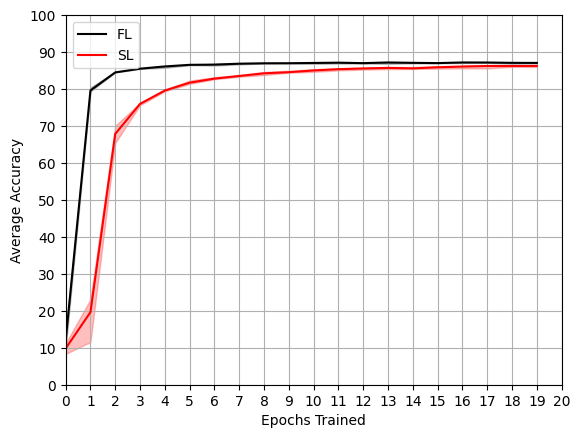
\includegraphics[width=300px]{aeg2}
	\caption{Comparing Accuracy of FL and SL with 1000 Data Samples per Node}
	\label{aeg2}
\end{figure}

In contrast to the observations in Figure \ref{aeg1}, it is apparent from Figure \ref{aeg2} that the training of \SL resulted in a comparatively lower accuracy. Additionally, \SL continues to exhibit a similar lag as before. There is also an overall decrease in accuracy for both methods, which can be attributed to the reduction in data.

\begin{figure}[H]
	\center{\textbf{Accuracy by Training Step for 100 Samples}} \\
	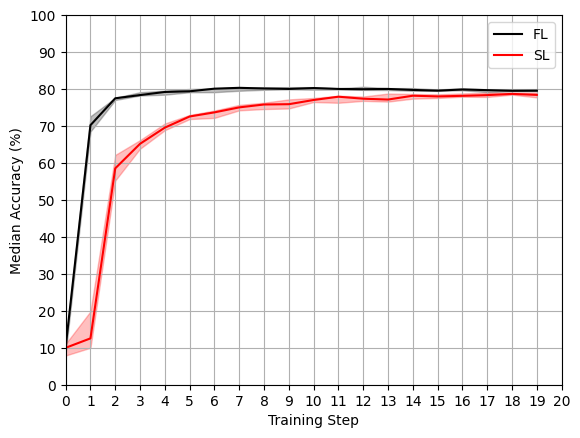
\includegraphics[width=300px]{aeg3}
	\caption{Comparing Accuracy of FL and SL with 100 Data Samples per Node}
	\label{aeg3}
\end{figure}

The trend of \SL ending with a lower accuracy than FedAvg continues in Figure \ref{aeg3}. Both algorithms also have a much lower accuracy than what they achieved previously, due to the drastic decrease in available data.

Similarly to Figure \ref{aeg2}, Figure \ref{aeg3} shows that \SL concludes with a lower accuracy than FedAvg. Furthermore, both algorithms exhibit a considerable decline in accuracy when compared to their previous performances with higher volumes of data.

\subsection{Analysis}

The most noticeable impact resulting from reducing the volume of data is the significant decrease in the accuracy of both algorithms, as expected. Nevertheless, it is also evident that the reduction in data affects \SL slightly more than FedAvg, as indicated by its progressively declining peak accuracy. Despite this, the difference in peak accuracy between the two algorithms remains quite small, often within a 2 percent margin.

One of the prominent challenges associated with \SL is its slower convergence rate compared to FedAvg, particularly from the outset. \SL consistently takes a longer time to attain its peak accuracy. This may be attributed to the asynchronous nature of the nodes in \SL, which implies that some nodes that conduct training before others may have lower accuracy than expected.

It is worth noting that in all these evaluations, \SL has a higher inter-quartile range than FedAvg, indicating that FedAvg is more consistent in terms of accuracy. However, this difference is minor.

\todo{Overfitting?}

\section{Dense Network Performance with Node Dropout}

\todo{Do this experiment - it really shouldn't take tong}

the same but this time dropout nodes. Try with and without filtering to show that it increases fault tolerance

To do this, test where a certain number of nodes drop out at step 1, 2, 3, etc

\section{Dense Network Performance with Connection Dropout}

\todo{Do this experiment - it really shouldn't take tong}

the same but this time dropout connections. Try with and without filtering to show that it increases fault tolerance

To do this, test where a certain number of nodes drop out at step 1, 2, 3, etc

\section{Sparse Network Performance}
In reality, it is uncommon for each node to be linked with every other node. To simulate a more realistic scenario, a technique was employed to generate a network of nodes with a specific density. It is important to note that, moving forward, density refers to an artificial metric and is not associated with the physical definition of density. When density is set to 0, the network is minimally linked, meaning that each node has at least one indirect path to every other node, but the minimal number of connections required to accomplish this exist. When density is set to 1, all nodes are connected to one another in a dense fashion. Since this measure may not provide a straightforward indicator of network density, two additional metrics will be provided:  Mean Minimum Hops (MMH) and Mean Connections per Node (MCPN). MMH denotes the mean minimum number of transitions required to get from one node to another in the network. MCPN denotes the average number of connections a given node possess.

In order to conduct thorough testing on a variety of potential deployment scenarios, several different densities were tested for each count of data. The densities that were tested, along with their corresponding MMH and MCPN, are presented in Table \ref{sparsedensities}.

\begin{table}[H]
	\centering
	\begin{tabular}{l|l|l}
		Density & MMH & MCPN \\ \hline
		1 & 1.0 & 9.0 \\
		0.75    & 1.2 & 7.2  \\
		0.5    & 1.4 & 5.4  \\
		0.25    & 1.7 & 3.6  \\
		0    & 3.0 & 1.8  \\
	\end{tabular}
	\caption{The statistics for different density levels} \label{sparsedensities}
\end{table}

In order to assist the reader with visualizing the various density levels, some sample networks that were generated for each density can be found in Figure \ref{densefig}.

\begin{figure}[H]
	\centering
	\begin{subfigure}[b]{0.3\textwidth}
		\centering
		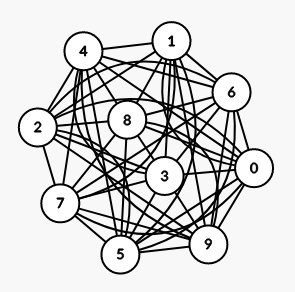
\includegraphics[width=\textwidth]{sparsegraph100}
		\caption{$density=1.0$}
	\end{subfigure}
	\begin{subfigure}[b]{0.3\textwidth}
		\centering
		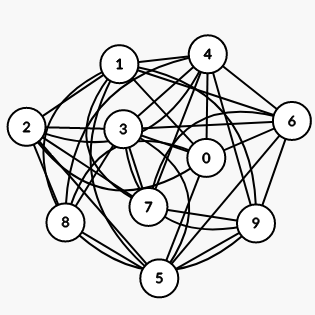
\includegraphics[width=\textwidth]{sparsegraph75}
		\caption{$density=0.75$}
	\end{subfigure}
	\begin{subfigure}[b]{0.3\textwidth}
		\centering
		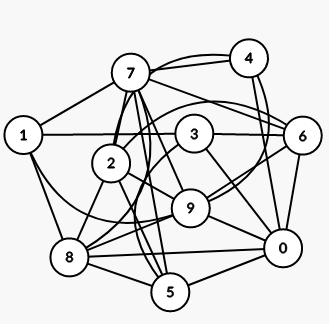
\includegraphics[width=\textwidth]{sparsegraph50}
		\caption{$density=0.5$}
	\end{subfigure}
	\begin{subfigure}[b]{0.3\textwidth}
		\centering
		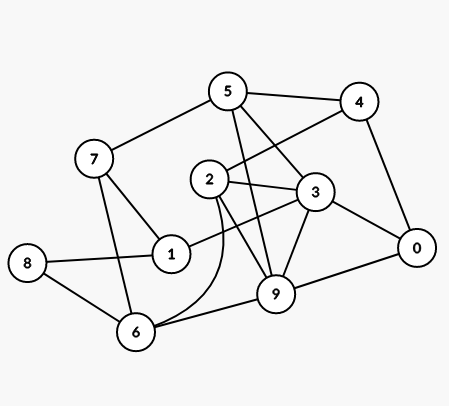
\includegraphics[width=\textwidth]{sparsegraph25}
		\caption{$density=0.25$}
	\end{subfigure}
	\begin{subfigure}[b]{0.3\textwidth}
		\centering
		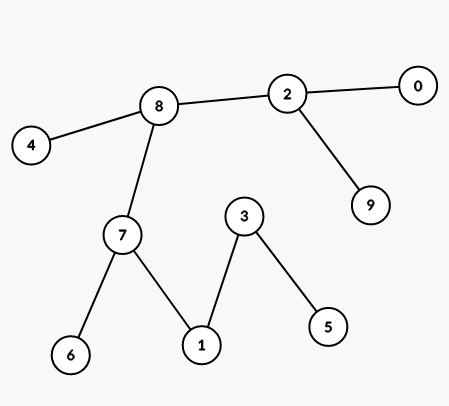
\includegraphics[width=\textwidth]{sparsegraph0}
		\caption{$density=0.0$}
	\end{subfigure}
	\caption{Example networks of nodes generated for each density level, visualised using the tool at \emph{https://csacademy.com/app/graph\_editor}. Each time a simulation is started, a new random network is generated for that simulation. \label{densefig}}
{}\end{figure}


This section does not include any testing of FedAvg. In scenarios where not every node is directly connected to the server node, FedAvg has two potential options: ignore all nodes which are not directly connected, or attempt to relay the model updates through connected nodes. As mentioned in Section \ref{relay}, relaying may not always be the optimal solution. Ignoring nodes is also not a good option, as data is wasted. Therefore, in this test, the decision was made to solely evaluate \SL.


\subsection{Results}
Presented below are the results obtained from executing the testing script. The density of each line on the graph is indicated by the color, with a green hue representing higher density and a red hue indicating lower density. For all tested densities, the value of $\gamma$ was set to $round_{down}(MCPN) - 1$, which ensures that each node can progress only after waiting for all but one of its neighbours. Notably, failure to reduce $\gamma$ for less dense networks would cause several nodes to wait for a number of neighbours that cannot be achieved. Due to the random nature of the graph generation, there will still be some nodes who do not have $\gamma$ neighbours, but this should be rare and the loop to wait for $\gamma$ neighbours will terminate after a certain number of tries anyway, ensuring that training can progress.

\begin{figure}[H] 
	\center{\textbf{Accuracy by Training Step for 6000 Samples for Different Densities}} \\
	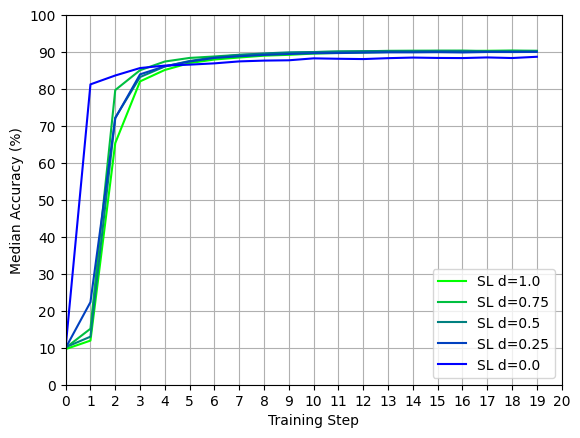
\includegraphics[width=300px]{aeg4}
	\caption{Comparing Accuracy of SL with 6000 Data Samples per Node and varying network density}
	\label{aeg4}
\end{figure}

It is noteworthy that among the 6000 samples tested, nearly all densities exhibited similar levels of performance, with the exception of density 0. Specifically, the densities achieved the same maximum level of accuracy and demonstrated comparable convergence rates. Although density 0 exhibited a faster convergence rate, its overall accuracy was lower than the other densities.

\begin{figure}[H]
	\center{\textbf{Accuracy by Training Step for 1000 Samples for Different Densities}} \\
	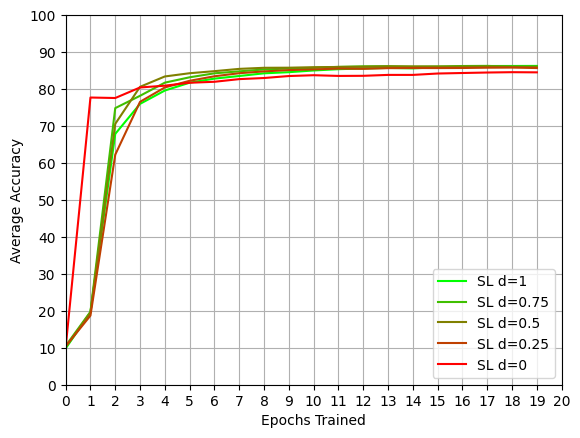
\includegraphics[width=300px]{aeg5}
	\caption{Comparing Accuracy of SL with 1000 Data Samples per Node and varying network density}
	\label{aeg5}
\end{figure}

The experiments conducted using a sample size of 1000 demonstrated comparable outcomes to those obtained with a sample size of 6000, albeit with a lower overall accuracy across all tests.

\begin{figure}[H]
	\center{\textbf{Accuracy by Training Step for 100 Samples for Different Densities}} \\
	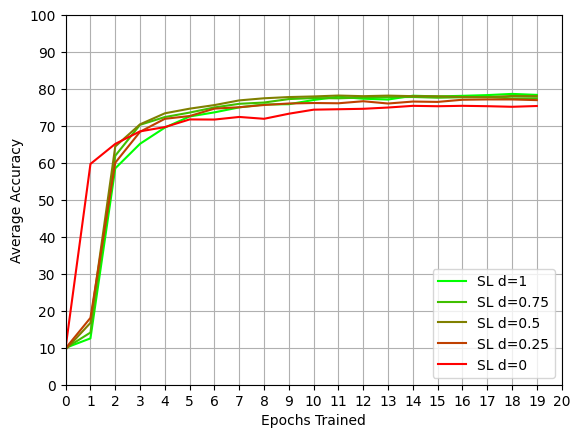
\includegraphics[width=300px]{aeg6}
	\caption{Comparing Accuracy of SL with 100 Data Samples per Node and varying network density}
	\label{aeg6}
\end{figure}

With only 100 training samples, it is evident that the network's density has a significant impact on the resulting accuracy. The final accuracy values span between 75 and 80 percent, with denser networks exhibiting higher accuracy rates. Additionally, the training curves depicted in Figure \ref{aeg6} appear to be more noisy compared to those obtained with larger datasets.

\subsection{Analysis}
In general, altering the network density of nodes has a small impact on the training of the nodes within the network. Decreasing the density of nodes typically leads to a lower final accuracy. This effect becomes more noticeable as the data volume provided to each node decreases, as demonstrated by the increased variability in training displayed in Figure \ref{aeg6} in comparison to Figures \ref{aeg4} and \ref{aeg5}.

The networks possessing a density of 0 attain their optima at a faster rate than those with higher densities. Figure \ref{aeg6} illustrates that the lower densities reach convergence marginally quicker than higher densities, yet are surpassed by the latter towards the end of training.